%%document
\documentclass[11.0pt]{article}
\usepackage[top=1.0in, bottom=1.0in, left=1.0in, right=1.0in]{geometry}
\usepackage{amssymb}
%%setup for figure environments and graphics
\usepackage{graphicx}
\usepackage{epstopdf}
\usepackage{multirow}
%captions 
\usepackage[textfont=it]{caption}
\usepackage[textfont=it]{subcaption}

%%Title and Author
\usepackage{authblk}% for correct display of affiliations 
\title{ Do Higher Housing Values Make Communities More Conservative? 
\newline Evidence from the Introduction of E-ZPass
\thanks{The authors thank Jeffry Frieden and Kenneth Shepsle for insightful comments. The authors names' are listed alphabetically, and the authors contributed equally to all aspects of the analysis. The usual disclaimers apply.}
}
\author[1]{ \sf Connor Jerzak}

\author[2]{ \sf Brian Libgober}

\affil[1]{ \sf Department of Government and Institute for Quantitative Social Science, 
\authorcr \sf Harvard University, 1737 Cambridge Street, Cambridge MA 02138
\authorcr  \sf e-mail: cjerzak@g.harvard.edu} 

\affil[2]{ \sf Department of Government and Institute for Quantitative Social Science, 
\authorcr \sf Harvard University, 1737 Cambridge Street, Cambridge MA 02138
\authorcr \sf e-mail: blibgober@g.harvard.edu}
\renewcommand\footnotemark{} %kills the * next to title in thanks
\renewcommand\footnoterule{}  %kills the * next to title in thanks


%%%Headers and Footers
\usepackage{fancyhdr,lastpage}
\pagestyle{fancy}

\lhead{\sf{  Jerzak \& Libgober  }}
\chead{}
\rhead{\sf{E-ZPass, Property Values \& Political Preferences} }
\lfoot{}
\cfoot{\arabic{page} }
\rfoot{}

\fancypagestyle{plain}{%
  \renewcommand{\headrulewidth}{0pt}%
  \fancyhead{}%
  \fancyfoot[C]{\footnotesize \thepage\ }%
}


%setup bibliography
\usepackage[backend=biber,style=alphabetic,citestyle=authoryear,maxcitenames=2,uniquename=false,uniquelist=false]{biblatex}
\bibliography{ConnorBrian.bib}

%
%%miscelaneous
\usepackage{nicefrac}
\usepackage{varioref} %for better cross referencing, using vref to include page numbers if not on same page

\begin{document}

\maketitle
\begin{abstract}
\noindent A rich corpus exists on the extent to which homeownership is central to American political attitudes. This paper contributes to the literature by using the introduction of E-ZPass in Pennsylvania and New Jersey to identify the effect of traffic-reducing transportation infrastructure on property values and, in turn, political behaviors. First, we develop a model showing that faster travel times results in individuals preferring a lower tax rate, as those who face the lower travel times are made effectively wealthier. Next, we present empirical evidence consistent with this theoretical result. We show that voting precincts near newly introduced E-ZPass toll plazas experienced a sharp increase in property values relative to similar precincts near non-E-ZPass exists, giving us leverage to identify the causal effect of property value changes on voting. After finding that the positive shock in property values is associated with a sizable increase in Republican vote share, we discuss the implications of this finding in light of the literature on homeownership and American politics. 
\end{abstract} 
\section{Introduction}

\section{Relationship to the Literature}
At least since the 1940s, social scientists have relied on survey research to understand the factors affecting voting behavior, yet only recently have scholars begun to use experimental and observational evidence to gain ``causal leverage for analyses of voting behavior'' \parencite{Bartels2010}. Early studies of voting behavior established that although individual vote choice is susceptible to election-year specific shocks (such as the presence of an unusually popular presidential candidate or war-time discontent), the way an individual votes in most elections is for the most part a function of their personal identity characteristics \parencite{Converse1966}. According to this line of research, the most significant determinants of long-term voting behavior include party identification, ethnicity, gender, age, religion, education, and occupation \parencite{Lazarsfeld1948,Berelson1954,Campbell1960,Stanley2006a}. Noteworthy too are the factors these studies did \textit{not} find significant for long-term voting behavior: preferences about political issues, for example, and economic self-interest. This is not to say that financial well-being was ever considered irrelevant for voting behavior; the literature is replete with studies demonstrating that the success of incumbents is tied to that of the economy \parencite{Tufte1975,Meltzer1975,Hibbs1987}. Yet this effect appears to be based largely on ``sociotropic'' evaluations of national economic performance, not personal economic experience, and evidence for the latter's effect on voting behavior is at best mixed, even in the short term\parencite{Linn2010}.  For early survey research, long-term voting behavior was for the most part reducible to an individual's demographic characteristics, and would not predict that increasing an individual's wealth or income would ipso facto change their vote choice.  This view is in considerable tension with formal models whose comparative statics expect such a relationship between an indivdual's economic situation and their voting behavior \parencite[e.g.,][]{Romer1975,Roberts1977,Meltzer1981}.

Although the conclusions of survey research just described have been replicated numerous times \parencite{Nie1976,Smith989,LewisBeck2008}, in the past decade these results have nonetheless faced significant challenges from scholars bringing to bear new data sources and applying new data analysis techniques. In particular, ideology and economic interest are gaining renewed recognition as determinants of life-long voting behavior. \textcite{Ansolabehere2008} show that the apparent incoherence of individual issue attitudes may largely be a result of measurement error, and that by averaging multiple question responses one gets a more stable estimate of individual issue attitudes, which become nearly as predictive of voting behavior as partisan identification.  \textcite{Gelman2007} use exit poll data to establish that income can be an important determiner of individual vote behavior, but its predictive power depends greatly on geography: in poor states like Alabama those who make little vote very differently from those who make a lot, while in rich states like Connecticut the difference is barely present. The primary innovation of both these papers is that they make compelling arguments for the use of data analysis techniques not normally used within the strand of survey research concerned with voting behavior.  Other recent papers have proposed to use entirely different data sources to explore questions about voting behavior that would have previously been answered with survey data alone. \textcite{Hersh2015}, building on the results of \textcite{Gelman2007}, use highly disaggregated registration, census, and election returns to show that income is a significant determiner of voting behavior only in Congressional districts with large minority populations. \textcite{Gerber2011} found a significant but ephemeral effect for televsion advertising by conducting a randomized experiment involving a \$2,000,000 ad-buy in a Texas gubernatorial race. \citeauthor{Arunchalam} use height as an instrument for studying the effect of income on support for the Conservative Party in the United Kingdom. \textcite{Ansell2014} looks at ANES survey data from individuals living in Metropolitan Statistical Areas for which the Federal Housing Adminstration collects data on home values to calculate the effect of home value appreciation on attitudes toward a redistributive program. Ansell's substantive results, that increasing property values makes individuals less likely to support redistribution, nicely compliment ours, especially since we do not rely on any of the same data sources and uses a different identification strategy.  This article continues in the vein of these most recent papers, using data sources and methods not frequently used in the voting behavior literature to support the claim that economic experience can have a significant effect on voting behavior. 

%textit{Works such as these  work places the common-sense notion that higher income individual typically support parties less supportive of redistribution helps to   diverse, well-identified studies establish that changes in income ca, which  work is encouraging given number of models that assume individual incentives.}



\section{Research Design}

%research design
In order to understand how changes in individual wealth affect voting behavior, we rely on the fact that the introduction of E-ZPass reduced transportation costs for some localities but not others. We propose IV and conditional difference-in-difference estimators to evaluate the change in political attitudes between precincts that were exposed to E-ZPass (and that thus experienced a rise in property values) and those that were not (Donald and Lang 2007). This shock is plausibly exogenous because E-ZPass plazas were not selected strategically at the time of introduction, but replaced already existing toll structures. We also perform a placebo analysis to ensure that the initial (endogenous) placement of the tolls does not confound our inferences.

\\ 
\indent We rely on a combination of low-level voting, political contribution, census and geographic data. All geographic analysis were conducted using ArcGIS with a national highway map provided by ESRI, the developer of ArcGIS. The location of E-ZPass tolling booths were taken from the replication dataset to \textcite{Currie2011a}, and this data was replicated and supplemented with data collected from Department of Transportation websites. 

We use three measures for Democratic support, our outcome of interest. First, we examine the two-party Democratic vote share in presidential elections. We define this quantity as the total number of votes cast for the Democratic candidate in each election divided by the sum of votes cast for either the Democratic or Republican candidate. Next, we also examine two-party Democratic cash share. This quantity is defined as the total dollar amount of campaign contributions given to the Democratic candidate for President divided by the total dollar amount contributed to either Republican or Democratic candidate. Finally, we also examine the support from stationary campaign contributors in 2000 and 2004. Stationary contributors are defined as citizens residing at the same address between election years, and who contributed to presidential candidates in both years. Here, we proxy for Democratic support in a precinct by dividing the number of stationary contributors supporting the Democratic candidate for President by the total number of stationary contributors there. Ideally, we would use party registration data from New Jersey and Pennsylvania to form a similar proxy of Democratic support. However, the 2000 voter files in these states were not available. Precinct-level data on the number of registered voters and the number of votes received by each party in Presidential elections, as well as shape files detailing the geographic boundaries of each precinct, were taken from \textcite{Ansolabehere2014}. Contribution data collected by the Federal Election Commission (FEC) was reported at the individual level by zipcode, and address information for contributors is available from \textcite{Bonica2013} as well. 

Census data used for matching and for obtaining home price statistics were taken from the 2000 decenial census and the 2005-2009 American Community Survey (ACS). Our matching variables are precinct-level statistics, and include average income, percentage of the population with a bachelors or professional degree, percentage of the population which identifies as black, percentage of the population which is female, percentage of the population which is over the age of 65, and percentage of the population residing in the same house as in 1995. 

Because these data are reported at different levels of aggregation, substantial effort was required to create a dataset suitable for analysis. Formally, we consider an observational unit in our study to be a voting precinct. Voting precincts are contiguous areas, typically cover about 5 square miles, and are roughly the same size as census block groups, the smallest area at which census data are reported. Zipcodes are usually larger areas containing multiple precincts or census block groups. Since the boundaries of precincts, census block groups, and zipcodes are generally not identical, we use areal interpolation to impute the data from these other geographic area to the precincts. ArcPython replication code is provided for those interested in seeing exactly how each column in our dataset was constructed. The intuition is no more complicated than taking a weighted average, with weights based on the amount of area that overlaps between the precinct and the other geographic area one is interpolating. Also crucial to our analysis is the distance of each precinct to the highway. For this purpose we consider the polling place as coded in \textcite{Ansolabehere2014} to be the precinct's location, and we operationalize distance to the highway (or an E-ZPass plaza) to be the minimum network or ``over-road distance" to the nearest highway entrance. 


Next, this analysis must address a key issue regarding internal validity. To obtain any causal estimate, it is first necessary to identify treatment and control groups, or at least some axis that is used to establish intensity of treatment and to enable researchers to compare units. However, studies that use geographic boundaries as identification mechanisms are open to criticism around how the treatment and control groups are specified. If the treatment and control groups can be defined arbitrarily, then a study may be vulnerable to criticisms over data mining. As a consequence, this analysis uses two definitions of treated and control groups in order to illustrate that our results are robust to a range of conceptual and empirical specifications. 

Our analysis first uses a conditional difference-in-differences (diff-in-diff) model with matching. This method takes as the treated group those precincts living close to an E-ZPass exit toll plaza, who therefore are more likely to have received an exogenous increase in their housing price. Whether ``close'' should mean 5, 10, or 15 miles is unclear \emph{a priori}, thus a sensitivity analysis is required to assess the dependency of the results on how one defines ``closeness.'' We must also define a reasonable control group that could have received a reduction in traffic but did not. To construct this control group, we examine precincts close to exits on major highways without E-ZPass tolls. However, particularly close to metropolitan areas, there are precincts that are both within 10 miles of an E-ZPass highway and 10 miles of a highway without E-ZPass.  In order to get genuine separation of treatment and control groups, we create a rule excluding those precincts that are in one testing group but are on the cusp of being on the other. The exclusion rule should have a radius at least as big as the inclusion rule to guarantee perfect separation. One should also be concerned that citizens may be willing to drive further to take a non-toll road than one with tolls (i.e. in citizens' everyday experience, perceived ``closeness'' to an E-ZPass exit may differ from perceived ``closeness'' to a non-E-ZPass exit). According to this line of reasoning, the radius of the exclusion rule should be a bit larger than the radius of the inclusion rule. If the exclusion radius is too large, however, one will exclude many units in metropolitan areas where different highways intersect. While, in principle, treatment and control groups could each have their own inclusion and exclusion rules, we assume that treatment and control each have the same rule for inclusion and the same rule for exclusion.  We conduct our basic analysis including a precinct in a testing group if it is within 12 miles of the highway it belongs in, but not within 18 miles of a highway it should not belong in. We then replciate the diff-in-diff on a grid of plausible values.

Our analysis next uses an instrumental variables (IV) approach. This method does not posit the existence of a separate treated and control group. Rather, we use distance to an E-ZPass toll plaza as an instrument for housing price appreciation for those precincts within some fixed distance from the toll plaza. This framework depends on two assumptions. First, distance to E-ZPass toll plaza must be correlated with the endogenous explanatory variable (i.e. gain in housing price). This correlation is strong (with a $t$-statistic of over $4$). Next, the instrument cannot be correlated with the error term of our explanatory equation predicting change in Democratic $2$-party vote share. This assumption would be violated if distance to E-ZPass toll plazas affected Democratic $2$-party vote share even when housing prices are kept constant. 

In what follows, we show that our results are robust to the specification of the treated and control groups, as well as to the method of inference. We have a slight preference for the conditional difference-in-difference approach because this specification of treated and control groups seems more natural. Areas $2$ vs. $10$ miles from an E-ZPass toll plaza may differ on unobservables to a greater degree than precincts near E-ZPass toll plazas and those near non-E-ZPass traffic exits. Even so, it is important to give careful thought to the specification of the treated and control groups in geographically-based analyses, and it is best to show the robustness of a result across a range of specifications.  We also take care to show that other important predictors of Democratic support do not undergo significant changes following the introduction of E-ZPass. 

%results
\section{Results}
\subsection{Conditional DD}

For the diff-in-diff analysis, our goal is to construct comparable treated and control groups. We do so by selecting precincts which are no more than a fixed distance away from E-ZPass or non-E-ZPass exits. Although it is reasonable to think of EZ-Pass introduction as an exogenous shock, independent of changes in Democratic vote share between the 2000 and 2004 elections, it is nonetheless still possible that the precincts we identify as ``treated'' systematically differ from ``control'' precincts near non-E-ZPass exits in terms of relevant background covariates. If this were to be the case, our estimates for the causal effect of E-ZPass might be partly confounded by the differing baseline characteristics of the treated and control groups. To protect against this possibility, we use matching to find a subset of the data that is well-balanced in terms of relevant covariates. Matching also reduces model sensitivity \parencite{Ho2007}, narrowing the range of estimated effects. In the matching routine, we use propensity score matching with a caliper of $0.20$. Matching was done without replacement. We also attempted Mahalanobis distance matching and coarsened exact matching, but these approaches gave poorer balance. Table~\vref{balance_table} presents summary statistics useful for analyzing covariate balance between matched units, while Figure~\ref{matches} presents a map showing which units have been placed in treatment and control. We find that treated and control communities are very similar on background covariates such as average income, percentage of the population over the age of 65, percentage of the population living in the same house as in 1995, percentage of the population which is female, and percentage of the population holding a bachelor's or professional degree. 





\begin{figure}[!htb]
    \centering
    \caption{Illustration of matches.  The tiles indicate change in democratic vote share between 2000 and 2004, with bluer areas resulting in a Democratic shift in vote share, and red a more Republican shift in vote share. The green boxes indicating treated units and brown shields indicating control.}
 \includegraphics[width=0.9\textwidth]{Figures/MatchesMap_final.eps}
\label{matches}
\end{figure}

\begin{table}[!htb] 
    \label{balance_table} 
    \centering  
\resizebox{\textwidth}{!}{\begin{tabular}{@{\extracolsep{5pt}} ccccccccc} 
\\[-1.8ex]\hline 
\hline \\[-1.8ex] 
& \multicolumn{2}{c}{\emph{Overall}} & \multicolumn{2}{c}{\emph{Treated}} & \multicolumn{2}{c}{\emph{Controls}} & \multicolumn{2}{c}{\emph{Difference}}\\
& \multicolumn{2}{c}{\textemdash} & \multicolumn{2}{c}{\textemdash} & \multicolumn{2}{c}{\textemdash} & \multicolumn{2}{c}{\textemdash}\\
 & Mean & (S.D.) & Mean & (S.D.) & Mean & (S.D.) & Dif. & (S.D) \\ 
\hline \\[-1.8ex] 
\emph{Average income} & \$61030.94 & (34783.57) & \$61497.61 & (30444.52) & \$60564.26 & (38642.63) & \$933.36 & (1235.67) \\ 
\emph{\% bachelors} & 16.3 & (9.3) & 16.37 & (8.5) & 16.23 & (10.03) & 0.14 & (0.33) \\ 
\emph{\% black} & 4.86 & (11.43) & 5.76 & (12.45) & 3.95 & (10.23) & 1.81 & (0.4) \\ 
\emph{\% professional degree} & 51.49 & (3.03) & 51.57 & (2.69) & 51.41 & (3.34) & 0.16 & (0.11) \\ 
\emph{\% female} & 15 & (6.94) & 14.98 & (7.67) & 15.03 & (6.13) & -0.05 & (0.25) \\ 
\emph{\% of pop. over 65} & 2.2 & (2.53) & 2.21 & (2.68) & 2.2 & (2.37) & 0.01 & (0.09) \\ 
\emph{\% in same house as in '95} & 62.66 & (11.73) & 62.67 & (11.56) & 62.65 & (11.91) & 0.03 & (0.42) \\ 
\hline \\[-1.8ex] 
\end{tabular}}
  \caption{Pre-treatment balance. Data from the 2000 Census. 
                           Sample size: 1324 treated and 1324 control
                           units.}
\end{table} 
    

Although our matching methods acheived balance on a number of covariates the literature has generally considered significant at predicting long-term voting behavior, treated units had an average African-American population of about 6\% while control units had an average African-American population of about 4\%. Because our $n$ is large, this difference was statistically significant. It is a concern, therefore, that changes in racial voting behavior between the 2000 and 2004 election could explain some of our results. The fact that the black population is so small in both groups decrease this possibility, however as a precaution we provide here a brief analysis of exit poll and turnout data for each state and each election year, in order to estimate how changes in African-American and non-African American voting behavior might effect our results. According to these exit polls, Gore was supported by 90.5\% of black voters and 51.4\% of other voters, while Kerry was suppoted by only 83.4\% of black voters and 47.3\% of other voters.\footnote{Here, all figures correspond to two-party vote, consistent with the approach taken throughout the paper. Individuals who say they supported Nader or some other candidate are therefore dropped in our analysis of these exit polls.}  At the same time, about 53\% of the black population and 56\% of the non-black population voted in 2000, while 61\% of the black population and 66\% of the non-black population voted in 2004. Assuming that these estimates of average turnout and support by race are the same in treated and control units, we can estimate the difference-in-difference in two-party vote share purely due to racial imbalance as being about -0.0007. \footnote{Formally, we use the following equation: $$(\frac{ T_B^{04} D_B^{04} +  T_O^{04}  D_O^{04}}{ T_B^{04} +  T_O^{04}} - \frac{ T_B^{00} D_B^{00} +  T_O^{00}  D_O^{00}}{ T_B^{00} +  T_B^{00}}) - (\frac{ C_B^{04} D_B^{04} +  C_O^{04}  D_O^{04}}{ C_B^{04} +  C_B^{04}} - \frac{ C_B^{00} D_B^{00} +  C_O^{00}  D_O^{00}}{ C_B^{00} +  C_B^{00}}) $$ 
Here, $T_B^{0X}$ is the fraction of the black population that voted in the year $200X$ multiplied by the fraction of the population that is black in the treated units, while $T_O^{0X}$ indicates the fraction of the population that voted among other races times the fraction of the population that is not-black.  $D_B^{0X}$, $D_O^{0X}$ indicates the proportion of blacks and non-blacks who supported the democratic Presidential candidate in year '$0X$. $C_B^{0X}$ is the fraction of the black population that voted in the year $200X$ multiplied by the fraction of the population that is black in the control units, with $C_O^{XX}$ is defined analogously.} Looking ahead, we will see that this is two orders of magnitude smaller than the effect we found. Thus, racial imbalance between treated and control does not seem to pose a serious threat to our analysis of voting behavior.

\begin{table}[!htbp] \centering 
  \caption{Difference-in-difference results for change in Democratic
    vote share. Matching/control variables include precinct-level covariates on average income, percent of residents living in the same house as in 1995, percent of residents who are black, percent of residents who are over the age of 65, percent of residents with a bachelor's degree. All matching/control data are from the US census.} 
  \label{voteshare_did} 
\footnotesize 
\begin{tabular}{@{\extracolsep{5pt}} cccc} 
\\[-1.8ex]\hline 
\hline \\[-1.8ex] 
 & Point Estimate & (Bootstrap S.D.) & (Block Bootstrap S.D.) \\ 
\hline \\[-1.8ex] 
Baseline model & -2.37 & (0.20) & (0.99) \\ 
\hline \\[-1.8ex] 
With covariate adjustment & -1.93 & (0.25) & (0.76) \\ 
\hline \\[-1.8ex] 
\end{tabular} 
\end{table} 

\begin{table}[!htbp] \centering 
  \caption{Difference-in-difference results for change in average home price. Matching/control variables include precinct-level covariates on average income, percent of residents living in the same house as in 1995, percent of residents who are black, percent of residents who are over the age of 65, percent of residents with a bachelor's degree. All matching/control data are from the US census.} 
  \label{homeprice_did} 
\footnotesize 
\begin{tabular}{@{\extracolsep{5pt}} cccc} 
\\[-1.8ex]\hline 
\hline \\[-1.8ex] 
 & Point Estimate & (Bootstrap S.D.) & (Block Bootstrap S.D.) \\ 
\hline \\[-1.8ex] 
Baseline model & \$81,785 & (4,868) & (17,580) \\ 
With covariate adjustment & \$68,237 & (5,039) & (12,485) \\
\hline \\[-1.8ex] 
\end{tabular} 
\end{table} 

\begin{figure}[t]
    \centering
    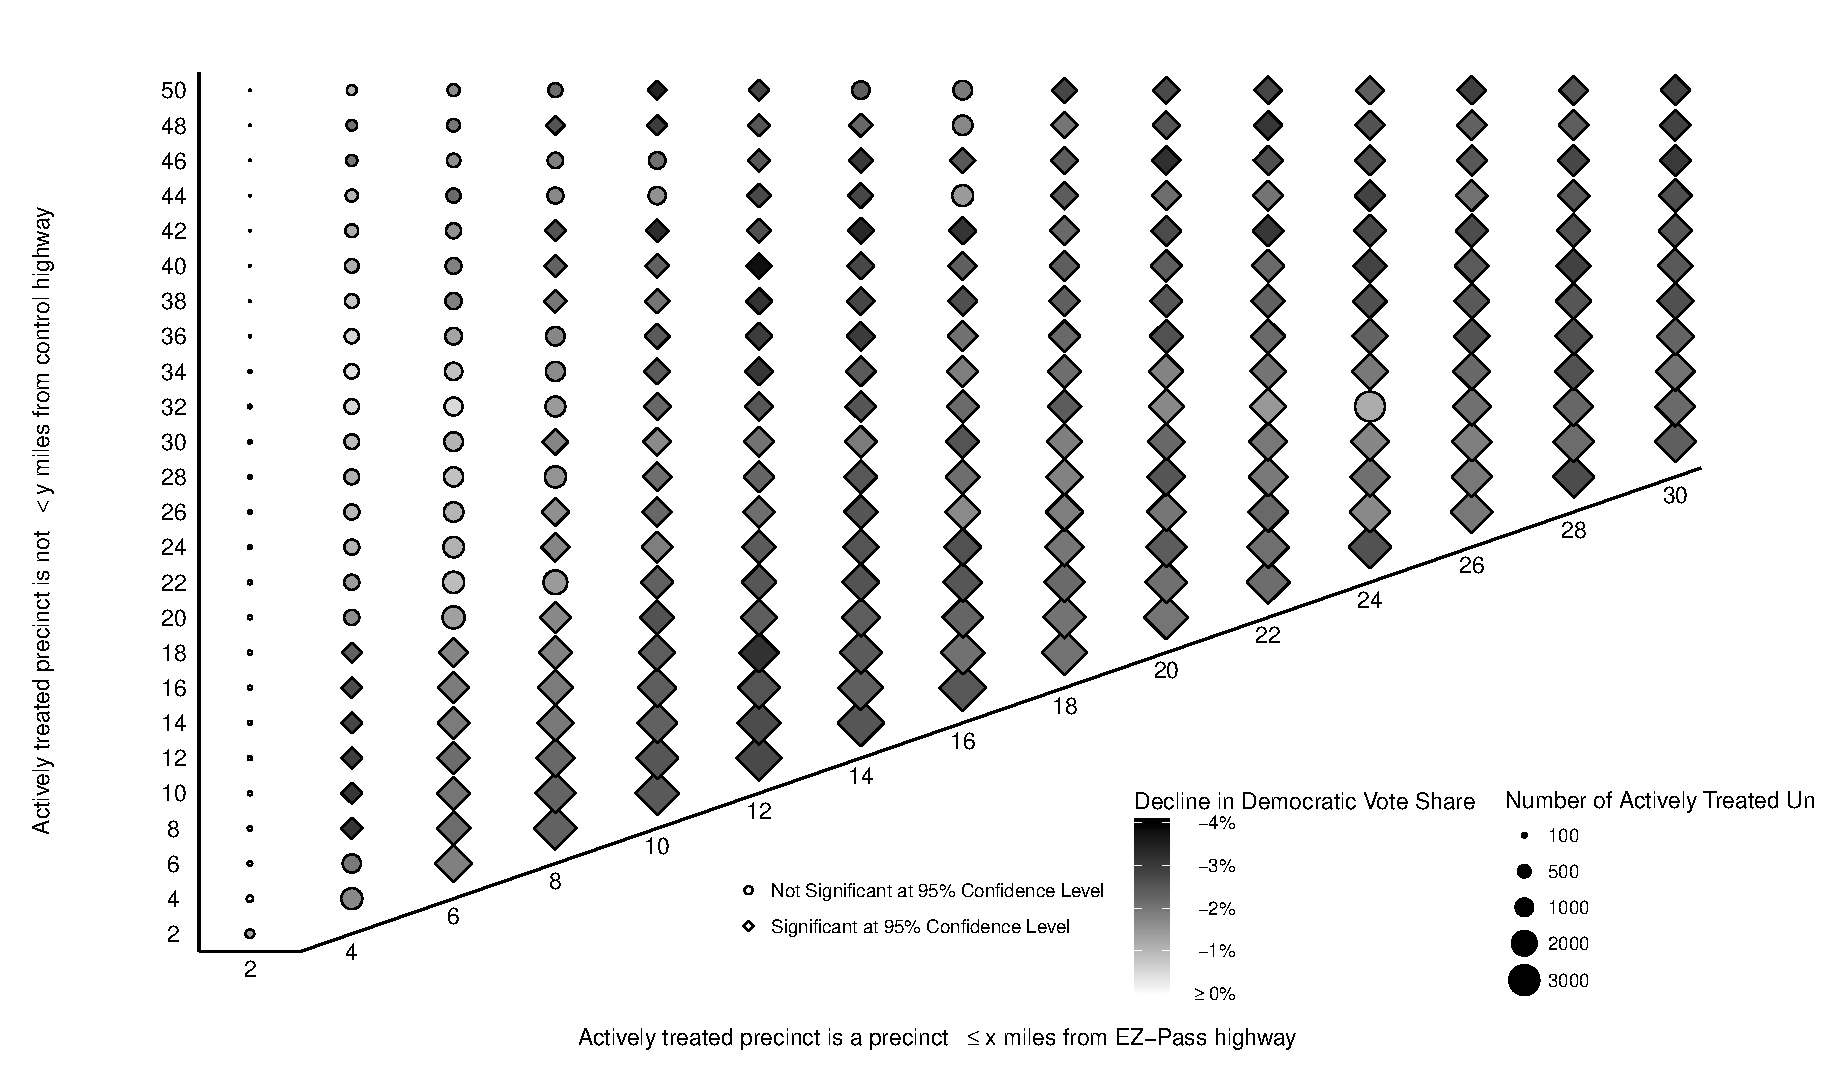
\includegraphics[width=0.9\textwidth]{Figures/new_style_04.eps}
    \caption{Sensitivity Analysis. $X$-$Y$ position gives the conditional difference in difference for a given combination of inclusion rule and exclusion rule. For example, at (12,18), one sees the effect of saying treated precincts are those within 12 miles of an E-ZPass highway but more than 18 miles from a non EZ-Pass highway, and similarly for control units. Effect size is indicated by the darkness of the shape, number of matched units is indicated by the area of the point, and results that are significant at the conventional 95\% threshhold are indicated by diamonds. Generally, effect magnitudes and significance are not sensitive to choice of rule, changes in effect magnitude are gradual.}
    \label{fig:heatmap}
\end{figure}
%threats to inferential validity
\subsection{Validity Checks}

Any diff-in-diff analysis is also threatened by the presence of time-varying confounders. The effect of the E-ZPass intervention might be correlated with other changes occurring in treated or control communities. Although we have little leverage in directly identifying unobserved confounding, we can establish empirically whether key observed confounders might be changing along with our outcomes of interest. In particular, we can identify such effects by completing the same diff-in-diff procedure for other factors that are important for predicting Democratic vote share. We find that no key predictors of Democratic vote share underwent changes associated with the introduction of the E-ZPass. 

Table \ref{alt_explanations} shows that average incomes seem to have remained stable in treated E-ZPass precincts relative to their control counterparts. The diff-in-diff estimate ranges from -$\$613$ to -$\$1,450$, but are statistically insignificant. We might have been concerned that E-ZPass might have pushed out poor residents and led to an influx of richer ones. However, this worry seems unfounded. Indeed, the sign suggests that incomes fell in E-ZPass precincts relative to control areas. Next, since E-ZPass precincts are now more desirable, it could be that these communities experienced an influx of new, potentially more conservative residents. However, we find that, on average, E-ZPass communities did not see a population change compared to the control areas. Changes in turnout might be another confounding variable. If E-ZPass significantly increase or decreased turnout, inferences about the changes in the average Democratic vote share might be suspect. Here too, we find no effect of E-ZPass. Finally, we might wonder whether other characteristics of the E-ZPass communities were affected by the introduction of the electronic tolls. Could it be that E-ZPass communities experienced changes in racial or educational composition? No, neither the percentage of black residents nor the percentage of residents with a bachelor's degree changed in treated relative to control precincts. 

\begin{table}[!tbp] \centering 
\caption{Diff-in-diff results for other key variables.}
\resizebox{0.95\textwidth}{!}{
\begin{tabular}{@{\extracolsep{5pt}} ccccc} 
\\[-1.8ex]\hline 
\hline \\[-1.8ex] 
& \multicolumn{2}{c}{\emph{Baseline model}} & \multicolumn{2}{c}{\emph{With covariate adjustment}} \\
& \multicolumn{2}{c}{\textemdash} & \multicolumn{2}{c}{\textemdash} \\
\hline \\[-1.8ex] 
Dependent variable & DiD Estimate & (Block Bootstrap S.D.) & DiD Estimate & (Block Bootstrap S.D.) \\ 
\hline \\[-1.8ex] 
\emph{Average income} & -613.81 & (2488.12) & -1830.39 & (2572.56) \\ 
\emph{Population} & 30.88 & (30.17) & 15.27 & (32.61) \\ 
\emph{Turnout} & 0.72 & (0.79) & 0.61 & (0.82) \\ 
\emph{Percent with bachelors} & 0.64 & (0.37) & 0.56 & (0.43) \\ 
\emph{Percent black} & 0.47 & (0.35) & 0.59 & (0.33) \\ 
\hline \\[-1.8ex] 
\end{tabular} 
} 
 \label{alt_explanations} 
\end{table} 


Although our matching methods acheived balance on almost all covariates the literature has generally considered significant at predicting long-term voting behavior, treated units had an average African-American population of about 6\% while control units had an average African-American population of about 4\%, and this difference was statistically significant. One concern is that changes in racial voting behavior between the 2000 and 2004 election could explain some of our results. The fact that the black population is so small in both groups decrease this possibility, however as a precaution we provide here a brief analysis of exit poll and turnout data for each state and each election year, in order to estimate how changes in African-American and non-African American voting behavior might effect our results. According to these exit polls, Gore was supported by 90.5\% of black voters and 51.4\% of other voters, while Kerry was suppoted by only 83.4\% of black voters and 47.3\% of other voters.\footnote{Here all figures correspond to two-party vote, consistent with the approach taken throught  the paper. Individuals who say they supported Nader or some other candidate are therefore dropped in our analysis of these exit polls.}  At the same time, about 53\% of the black population and 56\% of the non-black population voted in 2000, while 61\% of the black population and 66\% of the non-black population voted in 2004. Assuming that these estimates of average turnout and support by race are the same in treated and control units, we can estimate the difference-in-difference purely due to racial imbalance as -0.0007, two orders of magnitude smaller than our effect. \footnote{Formally, we use the following equation: $$(\frac{ T_B^{04} D_B^{04} +  T_O^{04}  D_O^{04}}{ T_B^{04} +  T_O^{04}} - \frac{ T_B^{00} D_B^{00} +  T_O^{00}  D_O^{00}}{ T_B^{00} +  T_B^{00}}) - (\frac{ C_B^{04} D_B^{04} +  C_O^{04}  D_O^{04}}{ C_B^{04} +  C_B^{04}} - \frac{ C_B^{00} D_B^{00} +  C_O^{00}  D_O^{00}}{ C_B^{00} +  C_B^{00}}) $$ 
Here, $T_B^{0X}$ is the fraction of the black population that voted in the year $200X$ multiplied by the fraction of the population that is black in the treated units, while $T_O^{0X}$ indicates the fraction of the population that voted among other races times the fraction of the population that is not-black.  $D_B^{0X}$, $D_O^{0X}$ indicates the proportion of blacks and non-blacks who supported the democratic Presidential candidate in year $XX$. $C_B^{XX}$ is the fraction of the black population that voted in the year $200X$ multiplied by the fraction of the population that is black in the control units, with $C_O^{XX}$ is defined analogously.}  Thus, racial imbalance between treated and control does not seem to pose a serious threat to our analysis of voting behavior.


Finally, because our data has a high degree of geographic correlation, it is important to consider other time-varying factors that might be confounding the analysis. While one cannot possibly hope to exhaust all such possible confounders, we do think it appropriate to consider one obvious confounder: weather. \textcite{Gomez2007} presents regression estimates of the effect of rain and snow on turnout and propoensity to vote Repbulican. They find that for every inch of rain above the normal amount of rain a place gets, there is on average about a 0.83\% decrease in turnout and about a 2\% increase in Republican vote. Since weather is also spatially correlated, it has the potential to confound the estimates for our vote share dependent variable (although not for our dependent variables based on donations). The perfect storm, so to speak, would be if it rained heavily along I-76 and I-95 (Southern Pennsylvania and Western New Jersey, respectively) in 2004, but nowhere else in 2004, and everywhere else in 2000. 

Fortunately, the perfect storm did not happen. Figure \ref{fig:precipitation} presents precipitation maps from November 7th, 2000 and Nov 2nd, 2004 as reported by the National Oceanic and Atmospheric Administration (NOAA). According to these maps, on election day 2000 there was about $\nicefrac{1}{100^{\mathrm{th}}}$ an inch of precipitation in Western Pennsylvania, while on election day 2004 there was about $\nicefrac{1}{4^{\mathrm{th}}}$ of an inch of rain in Western Pennsylvania, about $\nicefrac{1}{10^{\mathrm{th}}}$ of an inch in Central Pennsylvania, and a touch of rain around New York City. This is not a great deal of rain. Historical data available through Weather Underground characterizes conditions in the apparent epicenter, Pittsburgh, as ``light rain'' for most of the afternoon, cloudy in the morning and evening, with some additional rain around 9 pm. If one accepts the estimates in \textcite{Gomez2007}, the rain differential between 2004 and 2000 is not enough to make a significant dent in our estimates, even in a worst case analysis.\footnote{The normal rainfall in Pennsylvania is about 0.1 inches, so a worst case analysis that assumes 0.3 inches of rain in every treated unit but a normal amount of rain in every control would still only explain a 0.4\% increase in Republican vote. The effect we found was an order of magnitude larger. }  Moreover, the rain appears to affect treated and control regions evenly in 2004, if anything control regions were hit harder. To be especially sure that rain has not interfered with our inference, we estimate the effect on turnout due to E-ZPass. We find that there was no significant effect on turnout, which one would expect if rain was a serious confounder, and indeed the sign goes the opposite direction.

\begin{figure}[t]
    \centering
    \begin{subfigure}[b]{0.45\textwidth}
        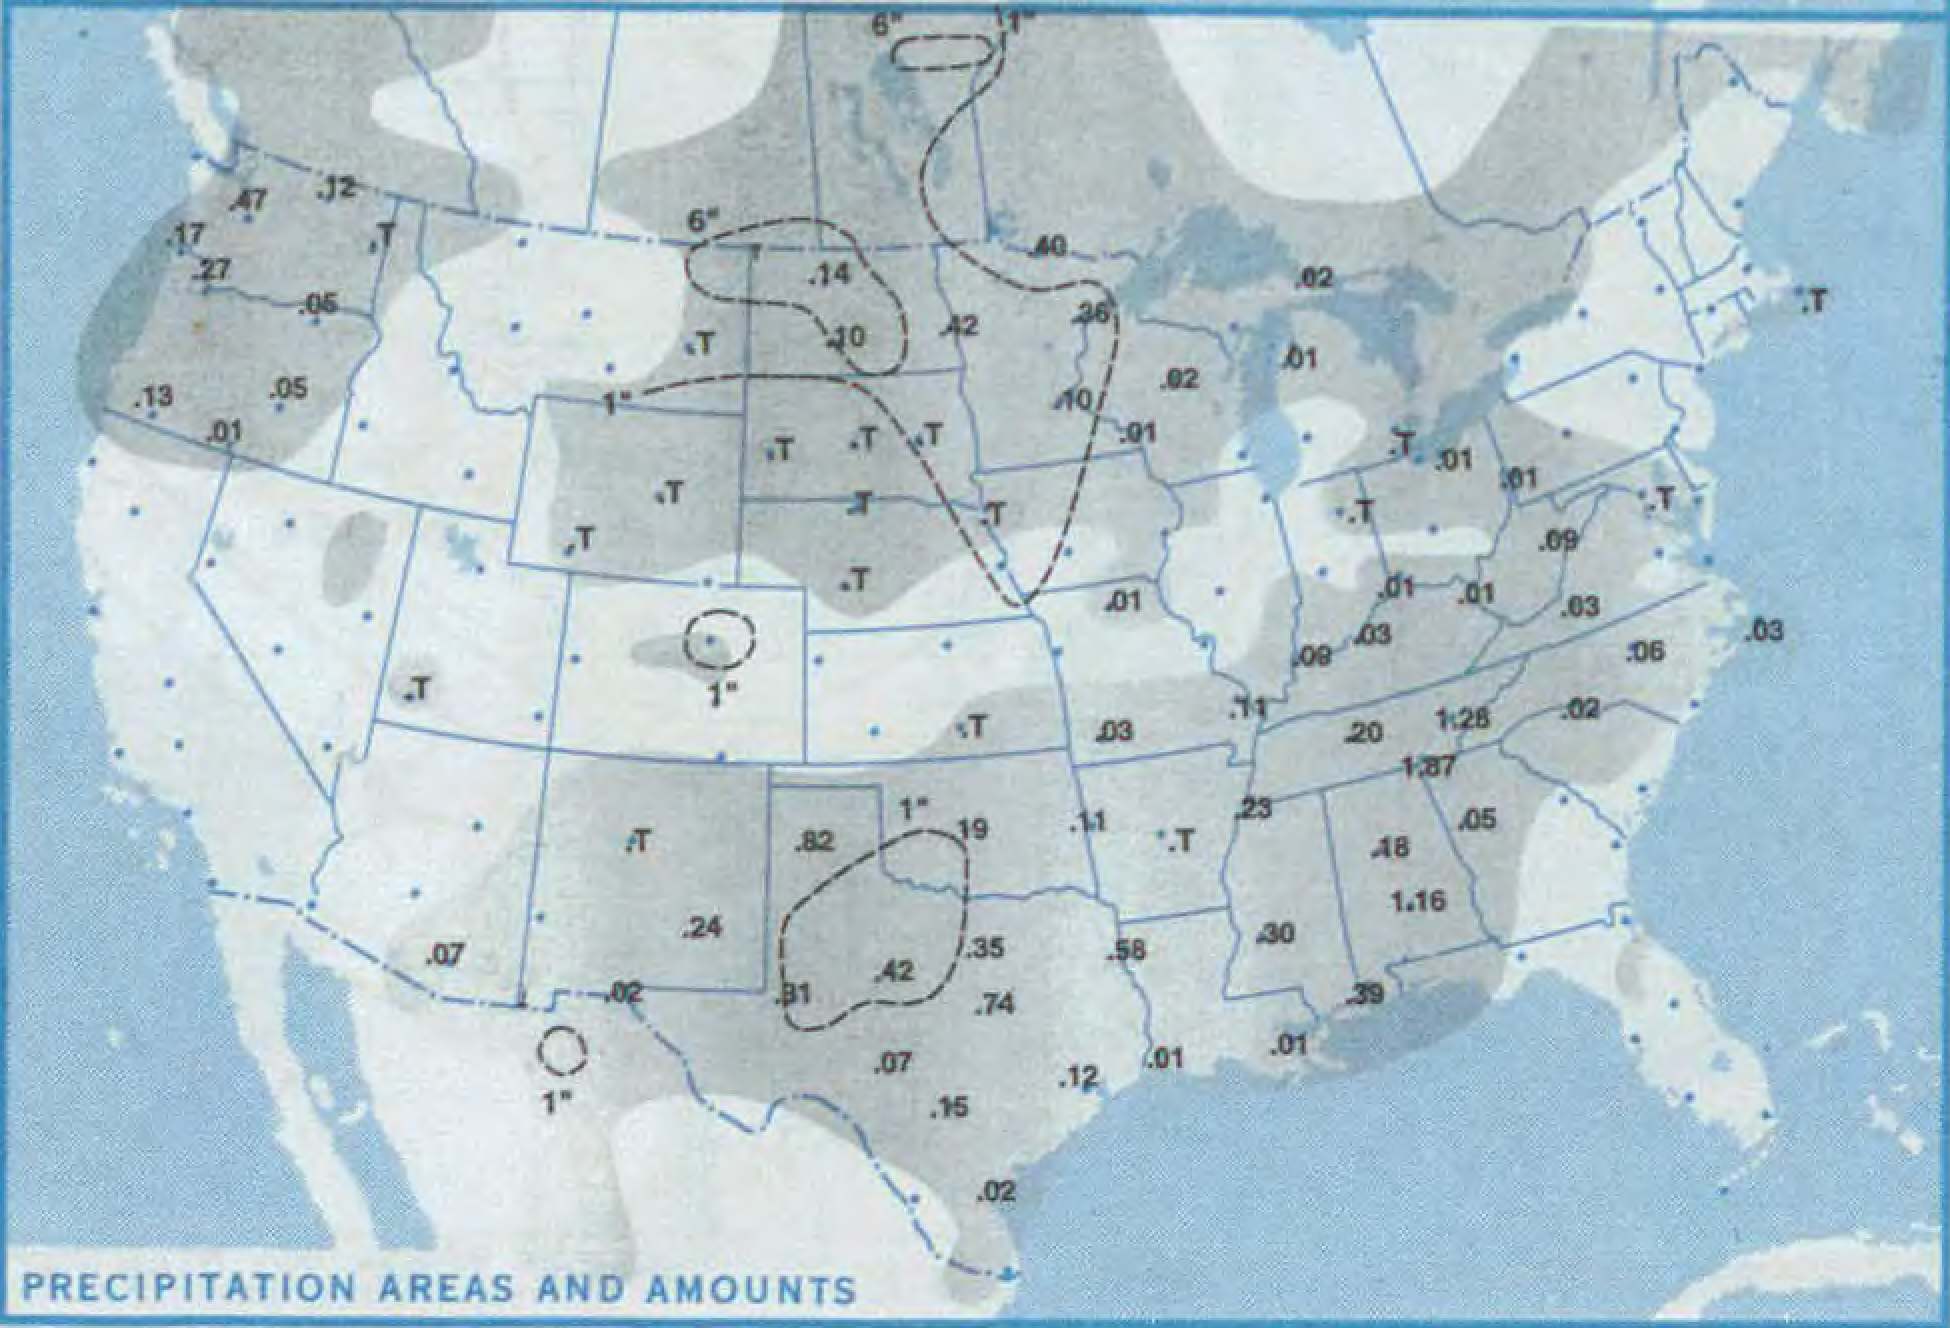
\includegraphics[width=\textwidth]{Figures/Election_2000_wednesday.png}
        \caption{7AM Nov. 7 - 7AM Nov. 8, 2000}
        \label{fig:gull}
    \end{subfigure}
    ~ %add desired spacing between images, e. g. ~, \quad, \qquad, \hfill etc. 
      %(or a blank line to force the subfigure onto a new line)
    \begin{subfigure}[b]{0.45\textwidth}
        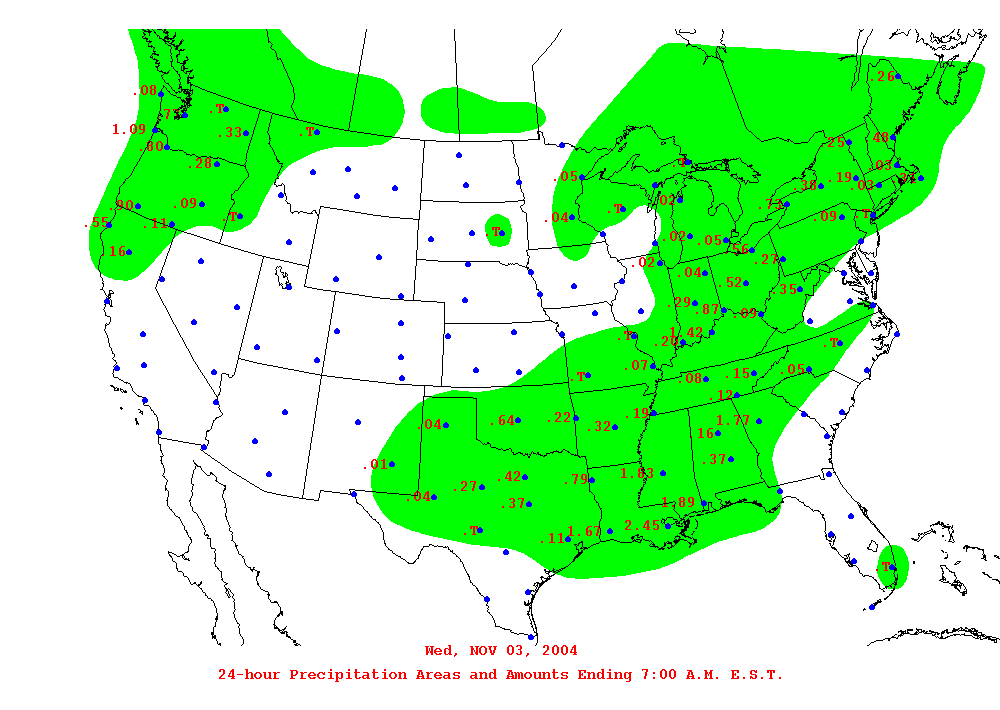
\includegraphics[width=\textwidth]{Figures/precip_20041103.png}
        \caption{7AM Nov. 2 - 7 AM Nov. 8, 2000}
        \label{fig:tiger}
    \end{subfigure}
    \caption{National weather maps from the two election days used in our study (Source: National Oceanic and Atmospheric Administration Central Library Data Imaging Project). The chart shows areas that had precipitation during the 24 hour period starting at 7 AM EST the day indicated until 7AM EST the next day. All numbers are reported in inches rounded to the nearest $\nicefrac{1}{100^{\mathrm{th}}}$, except for \textbf{.T} which refers to trace amounts of precipitation.}\label{fig:precipitation}
\end{figure}
\section{Conclusion}
This study has found that the introduction of E-ZPass brought about a significant rise in property values, and was also associated with a significant decrease in various measures of support for Democratic Presidential candidates. These relationships were estimated using conditional diff-in-diff and instrumental variables, techniques not frequently used in the study of political behavior. We have argued that this relationship between property values and support for Democratic candidates is causal, since EZ-Pass has not altered the environment in other ways that are significant enough to explain our results. 

Although our study has only looked at the introduction of EZ-Pass in the Eastern United States, the design is easily transported to other geographical contexts, both within the US and abroad. One interesting question for future research is whether the strength of the property-voting relationship depends on a community's wealth level. We have no real evidence to answer this question, but by analogy to income \parencite{Gelman2007}, we might expect the effect to be stronger in political communities that are poorer. Another important question is \emph{why} property values cause this effect. \textcite{Ansell2014} argues that a rise in property values gives individuals more ``permanent  income'' that can be converted via sale or borrowing, decreasing demand for social insurance. Others might argue that the effect is mostly due to the increased salience of property taxes. One could imagine a design that sought to sort out these explanations by using survey data rather than vote outcomes. The primary challenge for such a study is finding individuals who live close enough to a highway and therefore can be considered as participating in the study; if it were easy to find enough individuals using existing survey data, we would have done so. Yet with advance planning, such a study clearly could be done, since govermental entities typically announce EZ-Pass well in advance of installation. Such a panel survey might give political science scholarship additional causal leverage on the questions of how individual economic circumstances affect their attitudes. 
 
More broadly, we see our work as helping build an explanation for political polarization in the United States based on patterns of internal migration. Internal migration increases property values in states that gain citizens and decreases property values in states that lose them. The migrants themselves experience little change in individual wealth, at least in the short-term. However, those who already own homes in net recipient states should receive a windfall in their individual wealth. In the United States, migrants are predominantly leaving blue states and going to red states. Thus, internal migration has the effect of gradually making red states purple via a composition change, while pushing the already conservative home owners in red states even further to the right. More works needs to be done to evaluate such a theory, which we can only sketch in brief here. 

In sum, this work has used a novel identification strategy to address an important question at the intersection of political behavior and political economy. It suggests that scholars and political observers should consider citizens' entire economic portfolio, and not just income, in analyzing American politics. \hfill $\square$ 
\input{Sections/Appendix.tex}
\nocite{*}

\end{document}
